   \frame{
  \frametitle {A web server using docker}
	This requires the following tasks:\vspace{0.4cm}
	\begin{itemize}
	\item Download \textbf{\color{NavyBlue} nginx} docker image;\vspace{0.2cm}
	\item Execute this image using  the option \emph{\color{PineGreen}-p 80:80} to inform Docker that we want to expose the port 80. 
	\end{itemize}	  
  
    }
    
\frame{
\frametitle{A web server using docker}
    	\begin{center}
  			
\includegraphics[width=0.50\columnwidth]{./Figure/nginx}
  		\end{center} 

\begin{itemize}
\item It is a HTTP server software with focus on core web server and proxy features;\vspace{0.2cm}
\item It was developed to provide   high concurrency, high performance and low memory usage;\vspace{0.2cm}
\item It is able to scale incredibly far with limited resources.
\end{itemize}
}  
   \frame{
  \frametitle {Download nginx docker image}
  \begin{itemize}
  	\item Download nginx image;   	 
  	\end{itemize}
  	          	\begin{center}
  			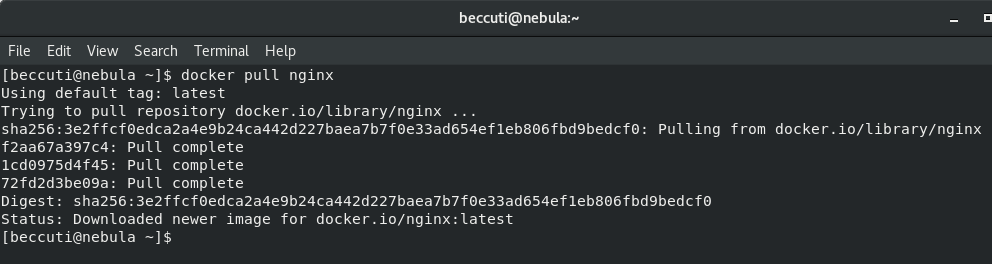
\includegraphics[width=1.0\columnwidth]{./Figure/pullnginx}
  		\end{center}	
  		
	
  		} 
   
 	     \frame{
\frametitle{Execute nginx docker image} 
  
 \emph{\color{PineGreen} docker run -p 80:80 nginx} must be used to star our web server on port 80.
     	\begin{center}
  			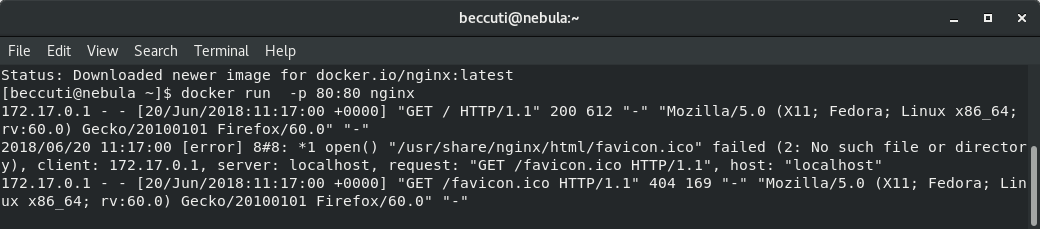
\includegraphics[width=1.00\columnwidth]{./Figure/runnginx}
  		\end{center}  
  	\begin{center}
  			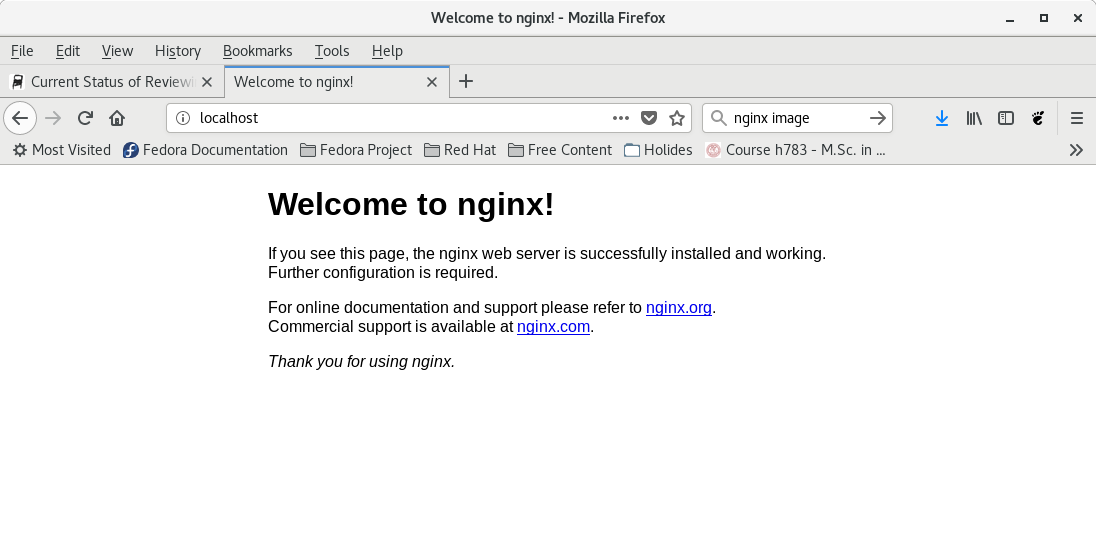
\includegraphics[width=0.95\columnwidth]{./Figure/webnginx}
  		\end{center} 
 }  	
 
   \frame{
\frametitle{Execute nginx docker image}

\textbf{\color{NavyBlue}How to use nginx to visualize fastqc output:}
\vspace{0.4cm}
\begin{itemize}
\item Update nginx image with \textbf{\color{NavyBlue}vi} command;\vspace{0.2cm}
\item Modify   \textbf{\color{NavyBlue}/etc/nginx/conf.d/default.conf}  adding     \emph{\color{PineGreen}autoindex on;} in  \textbf{\color{NavyBlue}location /} block;\vspace{0.2cm}
\item Execute nginx mounting the folder containing fastqc output in \textbf{\color{NavyBlue}/local/shared/nginx/html}.
\end{itemize}  

    	\begin{center}
  			
\includegraphics[width=0.50\columnwidth]{./Figure/nginx} \hspace{0.5cm} 
  			
\includegraphics[width=0.15\columnwidth]{./Figure/QC}
  		\end{center} 
  		    
  	   }  
  
  
   \frame{
\frametitle{Execute nginx docker image} 	   
 \textbf{\color{NavyBlue}How to use nginx to visualize fastqc output:}
\vspace{0.4cm}
\begin{itemize}
\item Update nginx image with \textbf{\color{NavyBlue}vi} command;\vspace{0.2cm}
 \end{itemize} 	   
  	     	\begin{center}
  			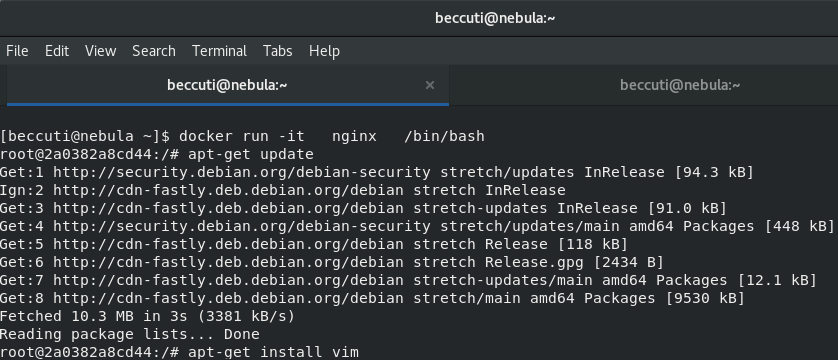
\includegraphics[width=1.0\columnwidth]{./Figure/vimnginx}
  		\end{center}  
  		}
  
    \frame{
\frametitle{Execute nginx docker image} 	   
 \textbf{\color{NavyBlue}How to use nginx to visualize fastqc output:}
\vspace{0.4cm}
\begin{itemize}
\item Modify   \textbf{\color{NavyBlue}/etc/nginx/conf.d/default.conf}  adding     \emph{\color{PineGreen}autoindex on;} in  \textbf{\color{NavyBlue}location /} block;\vspace{0.2cm}
 \end{itemize} 	   
  	     	\begin{center}
  			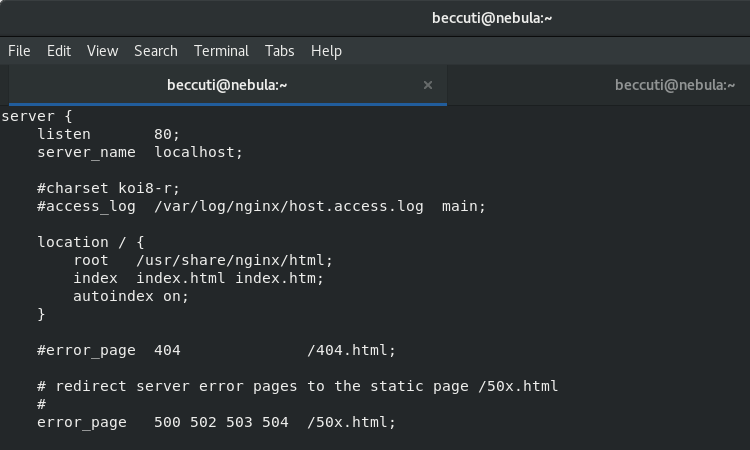
\includegraphics[width=0.90\columnwidth]{./Figure/confnginx}
  		\end{center}  
  		} 
  		
      \frame{
\frametitle{Execute nginx docker image} 	   
 \textbf{\color{NavyBlue}How to use nginx to visualize fastqc output:}
\vspace{0.4cm}
\begin{itemize}
\item Commit the updates in the images;
 \end{itemize} 	   
  	     	\begin{center}
  			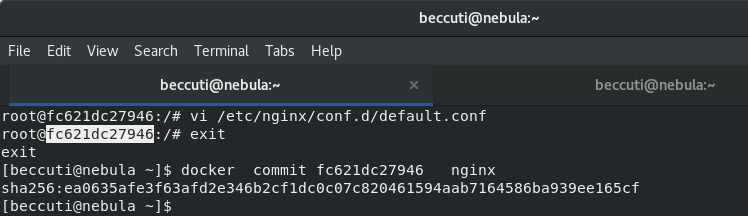
\includegraphics[width=0.90\columnwidth]{./Figure/commitnginx}
  		\end{center}  
  		} 
  		
  			
   		
      \frame{
\frametitle{Execute nginx docker image} 	   
 \textbf{\color{NavyBlue}How to use nginx to visualize fastqc output:}
\vspace{0.4cm}
\begin{itemize}
\item Run the new image \vspace{0.2cm}
\end{itemize}
  	     	\begin{center}
  			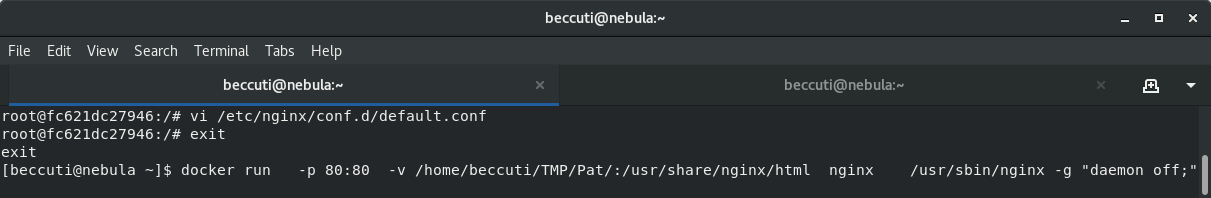
\includegraphics[width=1.0\columnwidth]{./Figure/run1ginx}
  		\end{center}
\begin{itemize} 		
\item Option \emph{\color{PineGreen}-v /home/beccuti/TMP/Pat/:/usr/share/nginx/html} is used to set the fastqc output folder as the root directory of web server;\vspace{0.2cm}
\item  Web server is executed in background  using \emph{\color{PineGreen} /usr/sbin/nginx -g "daemon off;"}.
 \end{itemize} 	   
  
  		} 
  		